
	%pi-calc commands
			
			
	\newcommand{\picalc}{%
		\texorpdfstring{$\pi$}{pi}-calculus}
	% \newcommand{\HUGE}{\fontsize{43}{54}\selectfont}
	% \newcommand{\PICALC}{%
	% 	\texorpdfstring{{\Huge{$\pi$}}}{pi}-Calculus\ %
	% }
	\newcommand{\exports}[1]{%
	\ensuremath{({#1})}%
	}
	\newcommand{\Picalc}{%
		\texorpdfstring{$\pi$}{pi}-Calculus}
	
	\newcommand{\send}[2]{%
	 	\ensuremath{{#1}!\langle{#2}\rangle}%
	}
	\newcommand{\sends}[2]{%
	 	\ensuremath{{#1}!{#2}}%
	}
	\newcommand{\ssend}[2]{%
	 	\ensuremath{{#1}!\langle{#2}\rangle.}%
	}
	\newcommand{\receives}[2]{%
	 	\ensuremath{{#1}?{#2}}%
	}
	\newcommand{\receive}[2]{%
	 	\ensuremath{{#1}?({#2}).}%
	}
	\newcommand{\receivenodot}[2]{%
	 	\ensuremath{{#1}?({#2})}%
	}
	\newcommand{\new}[1]{%
	 	\ensuremath{\text{new}({#1}).}%
	}
	\newcommand{\pif}[1]{%
		\ensuremath{\text{if } {#1}}%
	}
	\newcommand{\pthen}{%
		\ensuremath{\text{ then }}%
	}
	\newcommand{\pelse}{%
		 \ensuremath{\text{ else }}%
	}
	\newcommand{\comp}{%
		\ensuremath{\ |\ }%
	}
	\newcommand{\rec}[1]{%
		\ensuremath{\text{rec }{#1}.}%
	}
	\newcommand{\defequals}{%
	 \ensuremath{\overset{\tiny{def}}{=}}%
	}
	\newcommand{\encode}[1]{%
	 \ensuremath{\llbracket{#1}\rrbracket}%
	}
	\newcommand{\subst}[2]{%
	 \ensuremath{\llbracket{#1}/{#2}\rrbracket}%
	}
	\newcommand{\pdef}{\ensuremath{\Leftarrow}\ }
	\newcommand{\sys}[1]{\ensuremath{\mathbb{#1}}}
	\newcommand{\sequiv}{\ensuremath{\equiv}}
	\newcommand{\pred}{\ensuremath{\longrightarrow}}
	\newcommand{\evolves}[1]{\ensuremath{\overset{{#1}}{\longrightarrow}}}
	
	\newcommand{\preds}{\ensuremath{\cdotp\!\cdotp\!\cdotp\!\longrightarrow}}
	%end pi-calc commands
\documentclass[12pt,twoside]{reedthesis}
\usepackage{graphicx,latexsym} 
\usepackage{amssymb,amsthm,amsmath}
\usepackage{longtable,booktabs,setspace} 
\usepackage{url}
\usepackage{float}
\usepackage{natbib}
\usepackage{multirow}
\usepackage{datetime}
% \usepackage{a0size} used for a really big pi symbol - disabled

\usepackage[palatino]{quotchapwc} %figure out where to stick \thispagestyle{empty}%
\renewcommand\chapterheadstartvskip{\vspace*{-5\baselineskip}}
\usepackage[calcwidth]{titlesec}

%DIFFERING BEHAVOIR FOR PDF VS PRINT OUTPUT
\newcounter{outputmode}
\setcounter{outputmode}{0} %0 for pdf, 1 for print
\ifthenelse{\equal{\value{outputmode}}{0}}{\usepackage[bookmarks,unicode, colorlinks, linkcolor= darkblue, citecolor= darkblue, pdftitle={The $pi$-calculus}, pdfauthor={William Henderson}]{hyperref}}{\usepackage[bookmarks, colorlinks=true, linkcolor=black, citecolor= black, pdftitle={The $pi$-calculus}, pdfauthor={William Henderson}]{hyperref}}
\ifthenelse{\equal{\value{outputmode}}{0}}{\setlength{\evensidemargin}{0.3in}\setlength{\oddsidemargin}{0.3in}}{}

\titleformat{\section}[hang]{\sffamily\bfseries}
 {\Large\thesection}{12pt}{\Large}[{\titlerule[0.5pt]}]


\title{The \picalc}
\author{William Henderson}
% see http://library.reed.edu/help/thesisformat.html for formatting reqs
% The month and year that you submit your FINAL draft TO THE LIBRARY (May or December)
\date{May 2008}
\division{Mathematics and Natural Sciences}
\advisor{James Fix}
\department{Mathematics}

\setlength{\parskip}{0pt}

\begin{document}
	\lfoot[Build version: \pdfdate]{}%temporary - for revision marking
	\rfoot[]{Build version: \pdfdate}%
  \maketitle
  \frontmatter % this stuff will be roman-numbered
  \pagestyle{empty} % this removes page numbers from the frontmatter
    %!TEX root = /Users/will/Documents/Academic/MA 470 -THESIS/THESIS/thesis.tex
\chapter*{Acknowledgments}
\addcontentsline{toc}{chapter}{Acknowledgments}
I want to thank my hamsters, Boris Becker, and this bottle of Merlot.

\chapter*{Preface}
\addcontentsline{toc}{chapter}{Preface}
\section*{A Word About Formatting}
\addcontentsline{toc}{section}{A Word About Formatting}
One of the pedagogical aims of this thesis is to be as clear and reader-assistive as possible during its presentation.  To that end, I have taken several liberties in the formatting of this thesis.  Figures, equations, definitions, theorems and examples all share one numbering scheme in hopes that it will make them easier to locate. Where \defmargin{definitions} appear, they are clad in italics as well as in a margin box to make them easier to find.  Equation numbers also appear in margin boxes.  When \refmargin{definitions} definitions or equations are referred to later in the text, an assistive link will appear in the margin to avoid index-fingering.  To this end, the wired reader will note the presence within the backcover of a searchable pdf version of the text, wherein all references are hyper-textual (clickable).  The included CD also contains all the code referenced in this thesis.  

\chapter*{Abstract}
\addcontentsline{toc}{chapter}{Abstract}
In this thesis I will blow your mind, and possibly (hopefully?) my own in the process.

   	\tableofcontents
    \listoffigures
	\chapter*{Abstract}
The development of process algebras is of considerable interest in the study of distributed and mobile computation.  After considering the nature of distributed and mobile systems, we will look at two variants of the \picalc, a modern process algebra given by Milner, that can be used to model such systems.  We will then compare the expressive power of these calculi and explore the extent to which they can simulate one another.  Particular attention will be paid to the specific constructs wherein the calculi differ and whether and how these constructs represent behaviors found in real distributed and mobile systems.  

	%dedication?

  \mainmatter % here the regular arabic numbering starts
  \pagestyle{fancyplain} % turns page numbering back on

    %!TEX root = /Users/admin/Desktop/Documents/Academic/MA 470 -THESIS/THESIS/thesis.tex
\chapter{Introduction}\label{Introduction}
	Computer scientists have long been interested in algebraic models that are capable of describing computation by formulating a `program' as an algebraic expression along with a set of rules for reducing such expressions ---  i.e., `running' them.  
The advantage of such algebras is that they can be studied using formal reasoning techniques.  
This means that we can rigorously prove things about them and derive useful observations `programming' in them without ever having to actually implement them on a system.  
Of course, these algebras often are used in real languages whether faithfully or in part, but this is usually after they have been studied in detail for some time and we can be sure of their value.
	
	In the 1930s, Alonzo Church and Stephen Kleene introduced one such algebra, known as the\inidx{$\lambda$-calculus}.  
In the $\lambda$-calculus, we can write programs as expressions that are a series of nested functions, and we can run these programs by invoking the functions within.  
A function is indicated by the $\lambda$ symbol, followed by a single variable representing its input.  
For example, the following is a very simple `successor' program that takes in a number $x$ and adds 1 to it, returning the result:
	\[
		(\lambda x. x + 1)
	\]
To run this program, we need to actually apply it to something ---  that is, we need to give it input.  
We express this by placing the input to the right of the function, as in:
\[
	(\lambda x. x + 1) 4
\]
The above program first substitutes 4 in for the input $x$, yielding 4+1.  
The program then returns the result, 5.  
Since we can nest functions, a slightly more complicated version adds 1 to the input 4 and then multiplies the result by 3.  
We give this program with each computational `step' below:
\begin{align*}
	(\lambda y. y * 3) ((\lambda x. x + 1) 4)\\
	(\lambda y. y * 3) (4+1)\\
	(\lambda y. y * 3) 5\\
	5 * 3\\
	15\\
\end{align*}
You are probably already getting a sense of the expressive power of the $\lambda$-calculus.  
In fact, it is capable of expressing \emph{any} computer algorithm, even without the numbers and arithmetic operators we have implicitly included above!  Besides allowing us to study the nature of computation in the abstract, the $\lambda$-calculus went on to inspire many programming languages like Lisp, ML and Haskell, and even some functionality in languages like Smalltalk, Ruby and Python.
\section{Distributed Systems}
The discovery of the $\lambda$-calculus did not end the search for new algebras.  
More recently, new kinds of programs and demands have emerged with the computational platform of \defmarginwide{distributed systems}.
These systems consist of loose networks of machines capable of exchanging messages and information.  
We say this shared information and computational power belongs to `the system' in that any program running on the machines of the system can freely access these resources, coordinating efforts to produce a single complex behavior.
\begin{figure}[H]
\centering
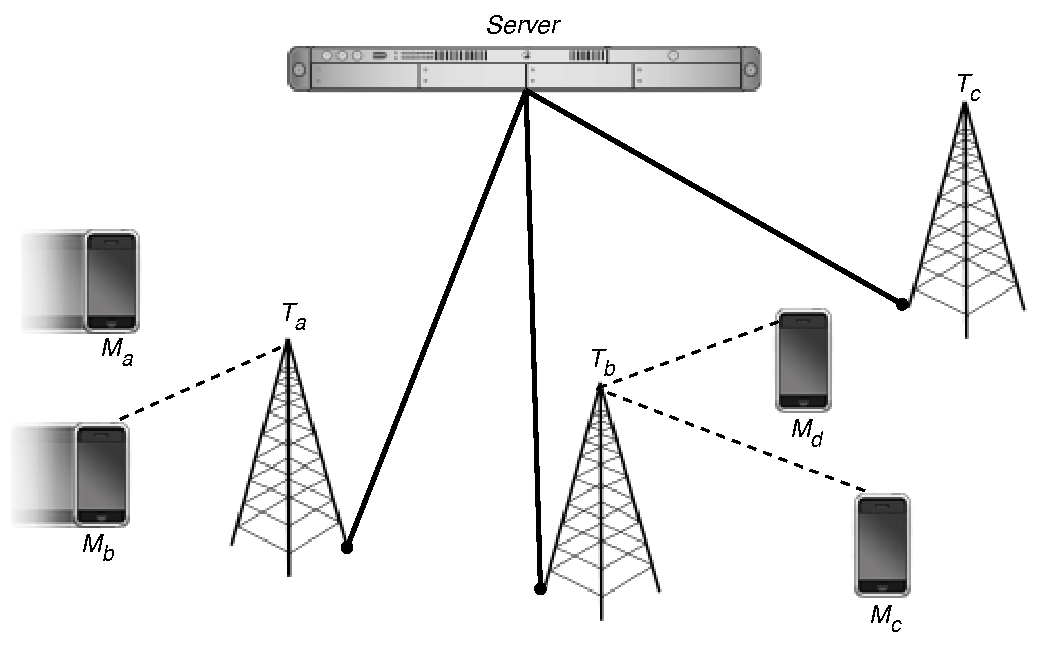
\includegraphics[scale=0.7]{figures/cell_network.pdf} % requires the graphicx package
\caption{\emph{A distributed mobile system}}
\label{fig_cell_network}
\end{figure}

For example, consider the familiar system that powers your mobile phone network.  
There may be one or more connected central servers, all of which are connected to the various towers that provide service.  
Towers and servers may have different capabilities and responsibilities, but the important thing is that the entire system needs to behave as a single unit with a network of shared information and computational power.  
A call in progress, for example, uses capabilities at various places in the system ---  on a tower to handle the call, on a server, perhaps, to handle the billing and routing of that call.  

Mobile clients are also connected and a part of this system.  
To place a call, for example, a user may use some capabilities on the phone to input the number, which is transmitted by the phone to the tower and then sent to the server to be routed.  
This entire `program' for making a call is one seamless operation that is happening across several machines.  

The demands of a distributed system strain the expressive power of the $\lambda$-calculus.  
Since the $\lambda$-calculus models all computation via functions, our only means of modeling a resource is as a function.  
Functions can only be accessed directly --- input can be passed to a function only by directly applying the function to that input.  
But if we want access to a resource on a system, we might not know where it is or what it is doing.  
Furthermore, our system of many machines could be doing many different things at once: routing calls, handling other calls in session, calculating a bill.  
Yet the $\lambda$-calculus has no means of easily expressing this concurrency which is so basic to many distributed systems.

Consider the phones on our system.  
They are \defmargin[mobile]{mobility} ---  in the sense that their connections to the system can be added and removed at any time.  
In \reffig{fig_cell_network} above, client $M_b$ is wirelessly connected to tower $T_a$ while $M_c,M_d$ are connected to $T_b$.  
Client $M_a$ is currently disconnected and $T_c$ has no clients.  
All the towers maintain a hard-wired link to the $\mbox{\emph{server}}$.  
We refer to the connections in a distributed system as its communication \defmargin{topology}.
$M_a$ and $M_b$ are in physical movement and their connections may change soon.  
$M_b$ might, for example, go out of range and disconnect from $T_a$ and connect to $T_b$ instead.  
Such changing communication topologies present even more difficulties to the $\lambda$-calculus.  
How can we abstract function invocation such that a function can be called from one place at one time, and another place later?  Even if we could somehow invoke a function indirectly, how could we deal with the fact that a function (say a client's ability to receive a call) is not currently available?

\section{Process Algebra}
Clearly we need an algebraic model for computation that eases the difficulty of modeling such systems.  \index{process algebra}
Such a model might consider computation via its natural distributed unit ---  the \defmargin{process}. 
A process is just a computational task, without reference to where it might be run nor with what input.  
For example, we could assign a process to a conversation on a phone somewhere in our network. 
Since\inidx{concurrency} of processes is such a basic operation, we make it a part of our algebra.  
A system, then, is simply a group of processes which are executing concurrently. 
Processes maintain computation state independently of one another.  
Instead of a single program state where functions interact via invocation, processes run independently and interact via \defmargin{message passing} --- sending data back-and-forth via named\inidx{channels}.  These channels can be shared between some or all processes in the system, but a single instance of communication is always between a pair of processes.

Because these channels can be shared among processes and used an arbitrary number of times, channels are not a concrete invocation system for a chunk of computation the way a function call is ---  processes simply send values to channels, assuming the receiver (if there is one) will do something useful with it.  
As with functions in the $\lambda$-calculus, processes are the basic unit of a program in process algebra. 
Any bit of functionality can be referred to as a process, with no specification of the granularity.

In 1978, C.A.R. Hoare introduced an early process algebra called Communicating Sequential Processes (\!\!\inidx{CSP})\cite{hoar78}.  In the 1980s, Robin Milner introduced his similar Calculus of Communicating Systems (\!\!\inidx{CCS})\cite{miln82}.  
 The CCS modeled systems as groups of communicating processes interacting via shared channels, and drastically eased the difficulty of modeling indirectly invoked concurrent operations.  
However, the CCS still would have had trouble with our mobile phone network, because it did not provide a way for processes to gain and lose their communication channels.  

	Although it can be defined in other ways, one of the ways of giving a process's\emph{\inidx{location}} is in terms of the communication channels which can be used to access it.  
Since processes are the units populating the space of a CCS system, it is natural to think of a process's location in terms of the processes which are `near' it ---  those it can connect to.  
Since communication happens via channels, a connection between processes just means that they share at least one channel.  
In this way, changing the communication channel topology of a system can be seen as changing the locations of its component processes.  

	In the CCS, channel topology is static ---  it does not allow new connections to be made or old ones to be removed.  
Not long after CCS's birth, Robin Milner, Joachim Parrow and David Walker created an improved algebra called the \inidx{\picalc}.  
The \picalc\ allows communication channels to be dynamically established and relinquished between processes.  
Since channels are what define location, dynamically created and destroyed channels give a kind of \emph{mobility} of processes, which vastly expands the capabilities of interaction in a system and finally allows us to give an account of our mobile phone system.
\section{The \Picalc: An Introduction}	
	As an example of how naturally the \picalc\ models distributed systems, let us again consider our mobile phone network\footnote{This presentation is adapted from a version first given by Milner \cite{miln99}}.  
Our system will be simplified a bit: only two towers and one phone, with the only system functionality being talking on the phone or switching from one tower to another.
	
	First we give a process describing the behavior of a mobile phone:
	\[
		Mobile(talk, switch) \pdef \ssend{talk}{} Mobile\langle talk,switch\rangle + \receive{switch}{t,s} Mobile\langle t,s\rangle
	\]
	Above, we use $\pdef$ to mean that the term to the right of the $\pdef$ is given the shorthand $Mobile$ and that refers the channels $talk$ and $switch$ defined elsewhere.  
When the shorthand is used, which occurs with angle brackets $\langle\rangle$, the channels given in the brackets are simply substituted for the terms in the parentheses.  
Hence, for example, $Mobile\langle talk_1,switch_1\rangle$ would be the right-hand term with the channels $talk_1$ and $switch_1$ substituted for $talk$ and $switch$. 
We call $Mobile(talk,switch)$ the \defmargin{interface} of the right-hand term.
	\begin{figure}[H]
	\centering
	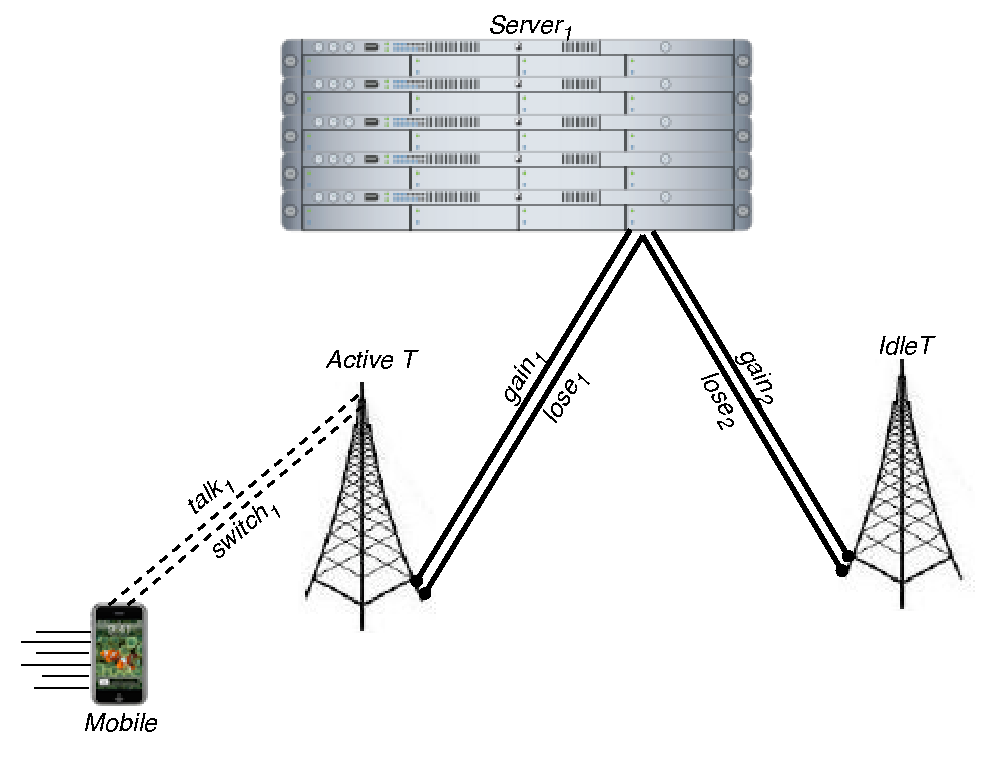
\includegraphics[scale=0.7]{figures/cell_network_pi.pdf} % requires the graphicx package
	\caption{\emph{Simplified mobile phone network in the \picalc}}
	\label{fig_cell_network_pi}
	\end{figure}
	The notation \send{talk}{} means that we are sending an `empty' (since there are no input values given in the brackets) signal on channel $talk$, while $\receivenodot{switch}{t,s}$ means we are listening on $switch$ to receive the input $t,s$.  
After a signal is sent or received on a channel, execution then continues with the term following the period, using the input provided (if any).
	Thus, $\receive{switch}{t,s} Mobile\langle t,s\rangle$ indicates that we should listen on $switch$ for the input $t,s$ and, when we receive it, use $t,s$ to `spawn' a new computation of $Mobile$ with these new channels. 
	The term $\ssend{talk}{} Mobile\langle talk,switch\rangle$ means send a signal on $talk$ before spawning a computation of $Mobile$ with the same $talk,switch$ channels we are using.  

Finally, the $+$ operator denotes that we should choose to compute one or the other of the operands (but not both).  
In sum, $Mobile$ has the ability to either send along $talk$ and stay in its current location, or it can receive over $switch$ and `move' to the location where it has new talking and switching channels $t,s$.  
This last capability expresses the mobile nature of our processes with surprising elegance: here we have just expressed that channels $talk,switch$ are dropped and new channels $t,s$ are established.
	
	Next we consider the behavior of a tower:
	\begin{align*}
		ActiveT(talk,switch,gain,lose) \pdef & \receive{talk}{}ActiveT\langle talk,switch,gain,lose\rangle \\  
		 & +\receive{lose}{t,s}\ssend{switch}{t,s}IdleT\langle gain, lose\rangle\\
		IdleT(gain,lose) \pdef & \receive{gain}{t,s}ActiveT\langle t,s,gain,lose\rangle\\
	\end{align*}
Here, there are two `states' our tower can be in.  
It can be active in talking with a mobile phone, or it can be disconnected and idle.  
If it is active, it can either receive over $talk$ (from the phone) and continue to be active, or it can receive over $lose$ (from the server, as we shall see below).  
In the latter case it then sends $t,s$ on $switch$ before becoming idle.  
That is, it will receive some new channels $t,s$ on $lose$ and then send them to the phone on $switch$ before becoming idle.  
An idle tower has only one capability: to receive over $gain$ and then become active again on the new channels $t,s$.

Finally we give the behavior of the server:
\begin{align*}
	Server_1 \pdef \ssend{lose_1}{talk_2,switch_2} \ssend{gain_2}{talk_2,switch_2} Server_2\\
	Server_2 \pdef \ssend{lose_2}{talk_1,switch_1} \ssend{gain_1}{talk_1,switch_1} Server_1
\end{align*}
Above, the server has two states: it can be controlling tower 1 or it can be controlling tower 2.  
In either case, the only capability is to lose one tower and gain the other before going into the opposite state.  
Hence, in $Server_1$ we can send to the first tower on $lose_1$ and then to the second tower on $gain_2$ before entering state $Server_2$.

We have now completely described the components of our system, but we still haven't put them all together.  
To do so, we'll need a new operator.  
This operator denotes that its operands run concurrently in parallel and is denoted $\comp$.  
Thus, our system is simply:\index{parallel}
\begin{center}
	\small{$\textstyle Mobile\langle talk_1,switch_1\rangle|ActiveT_1\langle talk_1,switch_1,gain_1,lose_1\rangle|IdleT\langle gain_2,lose_2\rangle|Server_1$}
\end{center}

\section{An Outline of This Thesis}	
	Now that we have gotten a taste of the power of the \picalc, we are ready to explore it in more detail.  
However, our first pass at the \picalc\ will not include some of the operators included in our mobile phone network example.  
For one, it will not include the $+$ operator\index{choice}\index{summation}.  
We will also use a version of sending that is a little simpler than the one we've seen so far.  
More specifically, our first calculus will be \defmargin{asynchronous}, meaning that processes will not continue on with any computation after sending on a channel.  
That is, in a process like
\[
	\ssend{c}{}P,
\]
we will disallow the presence of $P$ --- the process will simply terminate after sending on $c$.  
In Chapter \ref{the picalc}, we will give a rigorous presentation of the semantics of this asynchronous \picalc\ and the rules describing the way computation happens.

The two simplifications mentioned above will make our calculus somewhat easier to grasp, but there is another reason to consider an\inidx{asynchronous} calculus: it is far easier to implement on a real distributed system than the full synchronous version.  
At the base level, communication between machines on a distributed system is asynchronous, so implementing synchronous calculi requires finding a way to simulate synchronous message passing using only asynchronous primitives.  
In Chapter \ref{sync_and_express}, we will present the \defmargin{synchronous} \picalc\ (which has the full expressive power used in the mobile phone network example) and its computational rules.
Finally, Chapter \ref{sync_and_dist_sys} looks at the problem of modeling the synchronous \picalc\ using the asynchronous version.  It then takes a more practical-minded presentation of the way that a synchronous \picalc-like language might be implemented using asynchronous primitive \picalc\ constructs.
	
	%!TEX root = /Users/admin/Desktop/Documents/Academic/MA 470 -THESIS/THESIS/thesis.tex

\chapter{The \Picalc}\label{the picalc}	
	In this chapter, we will give the syntax of the \emph{asynchronous} \picalc\ and a discussion of its features.  
We will loosely follow the style of a recent presentation given in \cite{henn07}.  
Following this, we will introduce a notion of equivalence of terms in the language.  
Finally, we will give some semantic reduction rules that provide computational behavior via steps of reduction.
	\section{Syntax}\label{spisyntax}
	The terms of the \picalc\ operate on a space of \defmargin{identifiers} which consists of names $a,b,c,...,n,m,o$ for communication channels, and variables $v,w,x$ which can refer to channels, and recursive variables $p,q,r$, explained in more detail below.  
In general, we will use capital letter to denote a process.
	
		\begin{insettable}
		\begin{center}
		\begin{tabular}{r l l}
		\multicolumn{3}{c}{\emph{Process terms}}\\
		$R :=$  &$R_1 \comp R_2$ & Composition\\
		&\send{n}{\tuple{V}} & Send\\
		&$\receive{n}{\tuple{X}} R$ & Receive\\
		&$\new{n}R$ & Restriction\\
		&$\pif{v_1 = v_2}\pthen R_1 \pelse R_2$ & Matching\\
		&$\rec{p} R$ & Recursion\\
		&stop & Termination\\
		&\\
		
		\multicolumn{3}{c}{\emph{System}} \\
		& $\new{c_1,...,c_n} R_1 \comp...\comp R_m$ & $n, m >= 0$\\
		\end{tabular}
		\emph{\caption{Terms in the asynchronous \picalc}\label{apicalcterms}}
		\end{center}
		\end{insettable}
		\todo{Get index up to snuff by making sure more terms are margin defined.}
	Given two or more processes, we can compose them using the $\comp$ operator, which means that the composed processes will be executed concurrently.\index{parallel}
		
	\index{message passing}We denote the sending of a message $\tuple{V}$\index{tuple} over a channel $n$ by \send{n}{\tuple{V}}.  
Here $\tuple{V}$ is a tuple of identifiers in the form $\tuple{V}=(v_1,...,v_k):k\geq 0$.  
We say that $\tuple{V}$ has \defmargin{arity} $k$.  
In the case $k=0$ nothing is being transmitted; the communication acts as a \defmargin{handshake} or signal.  
We will denote this case by \send{n}{}.  
When $k=0$, only a single value $v_1$ is being transmitted, in which case we write $\send{n}{v_1}$.  
Because our calculus is \inidx{asynchronous}, sending is not a \defmargin{guarded} operation -- that is, a send operation does not continue to execute any process after sending its value, but simply terminates after sending the value.  
We will show in \refex{exsynchronous} that synchronous behavior can still be modeled in our language.
	
	The term \receive{n}{\tuple{X}}$R$ describes a process waiting to receive a tuple along $n$ before continuing with $R$.  
Here $\tuple{X}$ is a \defmargin[pattern]{patterns} -- a tuple of variables of arity $k$ -- which can be used anywhere in $R$.  
Patterns allow us to decompose the transmitted tuple into its component values by naming them with $x_1,...,x_k$, which can be referred to in $R$.  
Thus, in the term
	\begin{align}
		\send{c}{n_1,n_2,n_3} \comp \receive{c}{x_1,x_2,x_3} R,
	\end{align}
the names $n_1,n_2,n_3$ are received via $c$ and correspond to the variables $x_1,x_2,x_3$ in the pattern.  
 Hence, the variables $x_1,x_2,x_3$ can be used anywhere within the process $R$ to mean $n_1,n_2,n_3$.  


Similarly to sending, the case of arity 0 is denoted \receive{n}{}$R$ -- here $R$ will not happen until a handshake is received on $n$.  
Notice that in contrast to the case of sending, receiving is a \inidx{guarded} operation -- that is, the process $R$ will execute after $\tuple{X}$ has been received via $n$.  
For example, the term
\begin{align}
	\receive{c}{}stop
\end{align}
represents a `listener'	process that simply consumes the value waiting on input channel $c$.  
The term \emph{stop} describes a process that does nothing but halt.

	\index{scope restriction}The term $\new{n} R$ describes a process in which a new channel name $n$ is created and limited to being expressed in the process $R$ (we say the \defmargin{scope} of $n$ is \emph{restricted} to $R$).  
We shall see that scope plays a very big role in the way processes can establish new connections.  
Essentially, for a process $P$ to have a connection to another process $R$ really means that they both `know' about a common channel $c$.  
In that case, $c$ is scoped $P$ and $R$.  
Hence, $\new{n} R$ really means that we have created a channel $n$ that -- for the time being -- only process $R$ knows about.  
It is important to note that $n$ \emph{can} be used outside of $R$ if it is sent and then received by some outside process.  
This feature is known as \defmargin{scope extrusion}, and is the underpinning for the dynamic communication topologies introduced in the \picalc.  
For example, in the term
\begin{align}
	\new{n} (\send{c}{n}) \comp \receive{c}{x} \send{x}{},
\end{align}
	we have a channel $n$ scoped to the left hand process which is sending $n$ over $c$. The right hand process then receives $n$ over $c$ (referred to by $x$) and then sends an empty signal over $n$.  
At the time of its creation, $n$'s scope is just the left half of the term.  
However, after $n$ is received in the right hand process it will be able to be referred to outside of its initial scope.  
We will give a precise account of how this happens in our reduction rules and \refex{exscopeextr} below.
	
	We will sometimes abbreviate terms that use multiple channel restrictions by writing $\new{n,m}R$ to denote the term $\new{n}(\new{m}R)$. 
	
	Simple conditional execution based on value equality comparison is available through the use of $\pif{v_1 = v_2}\pthen R_1 \pelse R_2$.  
For example, in the following term, the value received on $c$ is checked; if it matches $a$ then a handshake is sent along $a$ (which is referred to by $x$), otherwise the process terminates.
	\begin{align}
		\receive{c}{x}(\pif{x=a} \pthen \send{x}{} \pelse stop)
	\end{align}
	
	Recursion is built into the language using the syntax $\rec{p}R$.  
The process $\rec{p}R$ itself is referred to by to the variable $p$, which is used somewhere in $R$ to express a recursive call.  
For example, consider the recursive responder term below, which receives a channel $x_1$ via $c$.  
It then sends a handshake response on $x_1$, while another responder process is run in parallel.
	\begin{align}
		\rec{p}\receive{c}{x_1}(\send{x_1}{} \comp p)
		\label{reclistenerterm}
	\end{align}
The variable $p$'s scope is restricted $R$, just as $X$ is restricted to $R$ in $\receive{c}{X}R$ and $n$ is restricted to $R$ in $\new{n}R$.
	
	We call a collection of parallel processes communicating over shared channels a\emph{\inidx{system}}.  
Note that a system is itself a process.  
  Our choice to define it is somewhat auxiliary to the \picalc\ itself, but it is helpful to understanding the way that behavior can be modeled using processes as atoms of a system.
\begin{example}{exsummation}
	 Many presentations (including our own in the next chapter) of the \picalc\ involve a \inidx{choice} or \inidx{summation} operator as in $P+Q$ for two processes terms $P$ and $Q$.  
The meaning is essentially that either $P$ or $Q$ can be non-deterministically executed, and the other process will not be.  
However, we can model the same behavior without defining a choice operator:
	\begin{align}
		\send{c}{} \comp \receive{c}{}P \comp \receive{c}{}Q
	\end{align}
	In the above process, either $Q$ or $P$ (but not both) could be executed.  
This is due to the asynchronous behavior of our language -- sending an empty signal along $c$, we cannot control which process consumes the signal (or even if it will be consumed at all). Thus, even without the choice operator our calculus is non-deterministic\index{non-determinism}.
\end{example}

\begin{example}{exsynchronous}
	 Perhaps we are not happy with this asynchronous transmission behavior.  
Surely we'd like to have blocking sends sometimes, or be able to guarantee that a value is received.  
Our asynchronous calculus can model \inidx{synchronous} sending by using a private channel that acknowledges when a value is received.  
To see how, consider the following system:
	\begin{align}
		F_1(c) & \pdef \rec{z} (\new{ack}(\send{c}{ack} \comp \receive{ack}{}(R \comp z)))\\
		F_2(c) & \pdef \rec{q} (\receive{c}{ack}(\send{ack}{} \comp q)) \\
		Sys_1 & \pdef \new{d}(F_1(d) \comp F_2(d))
	\end{align}
	Above, both $F_1$ and $F_2$ have (infinite) recursive behavior, and we can think of $Sys_1$ as a term that `kicks off' both of them after creating a shared channel for them to communicate on.  

	
	In an iteration of $F_1$, a new channel $ack$ is created for acknowledgement.  
This channel is sent along $c$ and then $F_1$ waits for input on $ack$ before executing some term $R$ and calling another iteration.  
$F_2$ receives $ack$ along $c$ and then uses $ack$ to send an empty signal to $F_1$ that it has received input on $c$.  

	
	This is just a toy example: the only thing being communicated is the acknowledgement channel itself.  
We might imagine a more complex system where $F_1$ sends more input along $c$ and waits to make sure $F_2$ receives it.  
Note that the channel $ack$ is only used \emph{once} -- we want to ensure that the acknowledgement that $F_1$ receives is definitely for \emph{that} instance of communication that it just initiated.  
This allows us to guarantee that $F_2$ has executed before $F_1$ continues with R.  
\end{example}

\section{Structural Equivalence}
	A natural question at this point is, given two \picalc\ terms, how can we determine if they are equivalent?  Intuitively, we want them to be equivalent if they \emph{act} the same, but actually defining this equivalence relation can be a bit subtle.  
In exploring this issue, we will first look at identifier substitution, giving rules for when we can safely interchange identifiers without creating a different term. Following this, we will develop the notion of \emph{contexts} and then use it to build an equivalence relation among processes.\index{equivalence}
\subsection{Identifier Substitution and $\alpha$-equivalence}\label{secSubst}
	As a first step in our notion of equivalence, we might assert that the way identifiers are named shouldn't change how they act.  
However, this doesn't mean we can start interchanging symbols with carefree abandon.  
In a component process, some terms might be important for how the process acts in a larger system.  
For example, if we changed the channel that a mobile phone uses to communicate with a tower, that phone certainly wouldn't act the same -- the tower would no longer know how to talk to it.  
On the other hand, we should be able to change any of the channels that the phone uses to communicate internally with itself without much issue.
	
	The only identifiers we can safely change in a process without potentially affecting the way it behaves in a larger system are \defmargin{bound identifiers}\refmargin{identifiers}.  
Intuitively, bound identifiers are those which are formally defined within the\inidx{scope} of the process.  
In a \picalc term there are three ways that identifiers can become bound.  
First, a name $n$ is bound in the process term $R$ to a new channel by the restriction operator as in \new{n}$R$.  
Second, each channel variable $x_i$ in the pattern $X$ is bound in $R$ to some channel $v_i$ from the sending process when matched in a receive expression \receive{c}{X}$R$.  
Finally, the recursive variable $x$ is bound in $R$ to process itself in the recursive expression \rec{x}$R$.
	\note{I choose not to give a recursive def'n here...we should talk about how to do this and whether it would be a good thing at this point of the discussion}
	We denote the set of bound identifiers in a term $R$ by $bi(R)$; all those which are not bound we call \defmargin[free]{free identifiers}, denoting them $fi(R)$.  
Similarly, we denote the set of bound and free names in a term $R$ by $bn(R)$ and $fn(R)$, respectively.  
We call a term with no free identifiers \defmargin[closed]{closed terms}.
	
	For example, in the term:
	\begin{align}
		\rec{p}\receive{c}{x_1}(\send{x_1}{} \comp p),
	\end{align}
	$p$ is a bound recursive variable, while $x_1$ is bound by the receive operator. The channel $c$ is free.  
Now consider the term
	\begin{align}
		\send{c}{n} \comp \new{n}(\rec{p}\receive{c}{x_1}(\send{x_1}{} \comp p))
	\end{align}
	Here $x_1, p$ are bound as before.  
However, the use of $n$ being sent on $c$ is \emph{not} bound, since it occurs outside the scope of the restriction operator.  
In fact, the following term (with the restriction operator removed) is equivalent (see \refex{exelimscoperest} for justification).
	\begin{align}
		\send{c}{n} \comp \rec{p}\receive{c}{x_1}(\send{x_1}{} \comp p)
	\end{align}
	When a receive term like $\receive{c}{X}R$ is executed, we substitute the free variables $\tuple{X}$ occurring in $R$ with the values $\tuple{V}$ that were received.  
We denote such substitutions by $R$\subst{\tuple{V}}{\tuple{X}}.  
During the course of a substitution, we might inadvertently `capture' a bound term.  
For example, suppose in the following term that some other process sent a channel $n$ over $a$ and that we wanted to perform the substitution \subst{n}{x} in running $\receivenodot{a}{x}$.\index{substitution}
\begin{align}
	P(a) \pdef \receive{a}{x}(\new{n}(\send{n}{} \comp \send{x}{}))
\end{align}	
The received term $n$ is not the same as the $n$ occurring in $P(a)$ - it was sent by some process outside the scope of the restriction operator $\new{n}$  Thus, the problem in performing $\subst{n}{x}$ is that it would make the free outside name $n$ into the bound name $n$.  
We say that running this substitution would \defmargin{capture} the bound name $n$.  
We can avoid this by first replacing the bound $n$ with a new name that is `fresh' -- that is it does not occur elsewhere in the term.  
For example:
\begin{align}
	P{'}(a) \pdef \receive{a}{x}(\new{n'}(\send{n'}{} \comp \send{c}{}))
\end{align}
We can now safely perform the receive and the corresponding substitution, yielding
\begin{align}
	\new{n'}(\send{n'}{} \comp \send{n}{})
\end{align}
	\note{again, I wanted to check in with you before defining Subst recursively}Obviously we want to say $P(a)$ and $P^{'}(a)$ are equivalent.  
In general when two terms are the same up to the use of bound identifiers, we say they are \defmargin[$\alpha$-equivalent]{$\alpha$-equivalency}, and write $P(a) \equiv_\alpha P^{'}(a)$.  
Thus, when we perform a substitution $R\subst{\tuple{V}}{\tuple{X}}$, we pick a term $\alpha$-equivalent to $R$ where the substitution will not capture terms bound in $R$.  
From now on we will intend that a term represents its entire $\alpha$-equivalency class, and thus will not explicitly specify $\alpha$-equivalency in the equivalence relation introduced below.

\subsection{Contexts and Equivalence}
Perhaps the next idea we might have for building our equivalence relation is that equivalent processes should act the same when dropped into any larger system.  
Let us define more precisely what we mean by `dropping in' a process.
\begin{definition}{Context}
	A context $\mathbb{C}$ is given by:
	\[
		\mathbb{C} := \begin{cases}
		[\ ]\\
		\mathcal{C} \comp Q \text{ or } Q \comp \mathcal{C} & \text{for any process $Q$, context $\mathcal{C}$}\\
		\new{n}\mathcal{C} & \text{for any name $n$, context $\mathcal{C}$}.
		\end{cases}
	\]
	$\mathbb{C}[Q]$ denotes the result of replacing the placeholder $[\ ]$ in the context $\mathbb{C}$ with the process term $Q$.
	\end{definition}
	Notice that with contexts, we do not pay any attention to whether a name in $Q$ is bound in $\mathbb{C}$.  
Hence, unlike with substitution, free variables in $Q$ can become bound in $\mathbb{C}[Q]$.  
So, for example, channel $c$ in the process $P(c) \pdef \receive{c}{}R$ can become bound in $\mathbb{C}[P(c)]$ where $\mathbb{C}[]$ is the context
\[
	\new{c}\send{c}{} \comp []
\]
We say that a relation $\sim$ between processes is \defmargin{contextual} if $P\sim Q$ implies $\mathbb{C}[P]\sim \mathbb{C}[Q]$ for any context $\mathbb{C}$.  
We are now ready to define our notion of equivalency using contexts.
	\begin{definition}{Structural Equivalence}
		Structural Equivalence, denoted $\sequiv$ is the smallest contextual equivalence relation that satisfies the following axioms:
		\begin{align*}
			P \comp Q\ &\  \sequiv\  Q \comp P && \text{\tiny{(S-COMP-COMM)}}\\
		 	(P \comp Q) \comp R\ &\ \sequiv\ P \comp (Q \comp R) && \text{\tiny{(S-COMP-ASSOC)}}\\
			P \comp \text{stop}\ &\ \sequiv\ P && \text{\tiny{(S-COMP-ID)}}\\
			\new{c} \text{stop}\ &\ \sequiv\ \text{stop} && \text{\tiny{(S-REST-ID)}}\\
			\new{c}\new{d} P \ &\ \sequiv\ \new{d}\new{c} P && \text{\tiny{(S-REST-COMM)}}\\
			\new{c}(P \comp Q)\ &\ \sequiv\  P \comp \new{c}Q\text{, if } c\not\in fi(P) && \text{\tiny{(S-REST-COMP)}}
		\end{align*}
	\end{definition}
	These axioms are simply a set of properties that we expect our syntax to obey.  
The first and second state that composition is commutative and associate.  
Thus, we will omit parentheses around compositions when our meaning is clear.  
(S-COMP-ID) states that a terminated process can be eliminated from a composition.  
(S-REST-ID) states that a channel scope restriction operator can be eliminated when its scope is only over a terminated process. (S-REST-COMP) states that scope ordering does not matter, justifying our shorthand $\new{c,d} P$.  
The last of these axioms is most important -- it is the basis for\refmargin{scope extrusion} \emph{scope extrusion}, upon which process\refmargin{mobility} mobility is based (as we shall demonstrate in \refex{exscopeextr} below).
	
	\begin{example}{exelimscoperest}
		In our discussion of bound identifiers above, we asserted that we can eliminate a scope restriction operation when none of the scoped identifiers occur in its scope. We can now show why this is permissible:
		\begin{align*}
			&\ \new{n,m}(\receive{a}{x_1,x_2}\send{x_1}{})\comp \rec{x}(\send{a}{n,m} \comp x) &&\\
			\sequiv\ &\ \new{n,m}(\receive{a}{x_1,x_2}\send{x_1}{} \comp stop)\comp \rec{x}(\send{a}{n,m} \comp x) && \text{\tiny{(S-COMP-ID)}}\\
			\sequiv\ &\ \receive{a}{x_1,x_2}\send{x_1}{} \comp \new{n,m}(stop)\comp \rec{x}(\send{a}{n,m} \comp x) && \text{\tiny{(S-REST-COMP)}}\\
			\sequiv\ &\ \receive{a}{x_1,x_2}\send{x_1}{} \comp stop \comp \rec{x}(\send{a}{n,m} \comp x) && \text{\tiny{(S-REST-ID)}}\\
			\sequiv\ &\ \receive{a}{x_1,x_2}\send{x_1}{} \comp \rec{x}(\send{a}{n,m} \comp x) && \text{\tiny{(S-COMP-ID)}}
		\end{align*}
	\end{example}
\section{Reduction Semantics}\label{secreducationsemantics}
We are now ready to give the \emph{semantic} properties that a process in our language should possess.  
By specifying the behavior of processes, we define how computation proceeds in the \picalc.  
The set of rules given below show how a process can internally evolve through a number of computation steps.\index{internal evolution}\todo{make all index terms lowercase}
\begin{definition}{Reduction}
	The \emph{reduction relation} \pred\ is the smallest contextual relation that satisfies the following rules:
	\begin{center}\begin{tabular}{rll}
		$\send{c}{\tuple{V}} \comp \receive{c}{\tuple{X}}R$\ &\  $\pred\  R\subst{\tuple{V}}{\tuple{X}}$ & \tiny{(R-COMM)}\\
		$\rec{x}R$\ &\  $\pred\  R\subst{\rec{x}R}{x}$ & \tiny{(R-REP)}\\
		$\pif{v = v}\pthen P \pelse Q$\ &\ $\pred\ P$ & \tiny{(R-EQ)}\\
		$\pif{v_1 = v_2}\pthen P \pelse Q$\ &\ $\pred\ Q$ \ \ (where $v_1\neq v_2$)& \tiny{(R-NEQ)}\\
		\multicolumn{2}{c}{\hspace{4.5em}$\underline{P\sequiv P', P \pred Q, Q\sequiv Q'}$} & \multirow{2}{*}{\tiny{(R-STRUC)}}\\
		\multicolumn{2}{c}{\hspace{4.5em}$P'\pred Q'$}
	\end{tabular}\end{center}
	We use the notation $P\preds Q$ when an arbitrary number of these rules have been applied in reducing $P$ to $Q$.
\end{definition}
The first of these allows a computation step for the transmission of values over a channel.  

(R-REP)  allows us to unravel a recursive expression into iterations of itself.  
(R-EQ) enables a computational step for value-matching.  
Finally, (R-STRUCT) says that a reduction is defined up to structural equivalence.
\begin{example}{exscopeextr}
	We will give a demonstration of how scope extrusion is defined using the rules and axioms of reduction and structural equivalence.  
Consider the expression 
\begin{align}
	\receive{d}{x}\send{x}{}\comp \new{c}(\send{d}{c} \comp \receive{c}{}stop)	
\end{align}
We can use (S-REST-COMP) to bring the restriction to the outside, giving:
\begin{align}
	\new{c}(\receive{d}{x}\send{x}{}\comp \send{d}{c} \comp \receive{c}{}stop)		
\end{align}
	Thanks to the reduction relation's contextuality, we can use (R-COMM) inside of the restriction operator and apply a substitution.  
Using this in conjunction with the above structural equality and (R-STRUCT), we get:
	\begin{align}
		\new{c}(\send{c}{} \comp \receive{c}{}stop)
	\end{align}
	Finally, we can apply (R-STRUCT) again, so the process simply reduces to stop.  


	Now let $P(d)$ to be the right half of our original process, and $\mathbb{C}$ to be the remaining context:
	\begin{align}
		P(d) \pdef \new{c}(\send{d}{c} \comp \receive{c}{}stop)
	\end{align}
	\begin{align}
		\mathbb{C} = \receive{d}{x}\send{x}{} \comp [\ ]
	\end{align}
Then we have shown that if we drop $P(d)$ into the context $\mathbb{C}$ (forming $\mathbb{C}[P(d)]$), it will establish a new channel $c$ and extend its scope using $d$.  
Hence it is (S-REST-COMP) which allows our system's communication topology to change dynamically via scope extrusion.
\end{example}
\begin{example}{exmemcells}
	Suppose we wanted to model a simple memory cell with channels for getting and setting its value.  
It turns out that we can simulate this just using message passing.  
The problem that we have to work around is that receiving a identifier from a channel removes that value from the channel -- it cannot be retrieved again.  
Thus, we need a way to push it back in for the next time.  
Consider the following system:
	\begin{equation}\begin{split}
		Cell(get,set) \pdef \new{c} & (\send{c}{init} \\
		& \comp\rec{g}(\receive{get}{b}\receive{c}{y}(\send{c}{y}\comp \send{b}{y}\comp g))\\
		&\comp\rec{s}(\receive{set}{x,b}\receive{c}{y}(\send{c}{x}\comp\send{b}{x}\comp s)))
	\end{split}\end{equation}
	In the cell, we first create a new channel $c$ that will be used to `store' the value.  
We then initialize $c$ with the value $init$.  
The following line has a recursive listener process than, when given a channel via $get$, gets the value from $c$ and sends it back via the supplied channel.  
In parallel, it sends the value back into $c$ so it can be had again.  
The next line is similar except that two values are supplied via $set$ - a new value and a channel.  
The old value is pulled from $c$ and simply discarded (ie not used), whereas the new value $x$ is pushed to the $c$ this time.  
$x$ is also sent via $b$ as an acknowledgment that the cell's new value has been set.
	
	Also notice that the system has the free channels $get_c,set_c$ given in the interface.\refmargin{interface}  When some larger system binds them and uses them to interact with the components inside $Cell(get_c,set_c)$ we say that the system \defmargin[instantiates]{instantiate} $Cell(get_c,set_c)$.  
In the following example we assume some larger system uses $printer$ to actually print the message.
	\begin{equation}\begin{split}
		Echo(printer) \pdef\\
		\new{get_1,set_1} & (Cell\langle get_1,set_1\rangle\\
		&\begin{split}\comp \new{a}(&\send{set_1}{``hello,\ world",a}\\
		&\comp \receive{a}{x}(\send{get_1}{a}\comp \receive{a}{y}\send{printer}{y})))\end{split}
	\end{split}\end{equation}
	The system $Echo$ creates new channels to interact with the instance of memory cell it spawns, while in parallel it puts a message in the cell, then (order is ensured using by waiting for the response via $a$) getting the value from the cell and sending it to the $printer$ channel.
	
	To see why this produces the behavior we expect, first observe scope restrictors for $a$ and $c$ can be moved out using $(S-REST-COMP)$:
	\begin{equation}\begin{split}
		\new{get_1,set_1,a,c} & \Big(\send{c}{init} \comp\rec{g}(\receive{get}{b}\receive{c}{y}(\send{c}{y}\comp \send{b}{y}\comp g))\\
			&\comp\rec{s}(\receive{set}{x,b}\receive{c}{y}(\send{c}{x}\comp\send{b}{x}\comp s))\\
		&\comp \send{set_1}{``hello,\ world",a}\\
		&\comp \receive{a}{x}(\send{get_1}{a}\comp \receive{a}{y}\send{printer}{y})\Big)
	\end{split}\end{equation}
	Two applications of (R-REP) allow us to `pull out' a recursive call:
	\begin{equation}\begin{split}
		&\new{get_1,set_1,a,c}\\
		&\Big(\send{c}{init} \comp\receive{get}{b}\receive{c}{y}(\send{c}{y}\comp \send{b}{y})\comp \rec{g}(\receive{get}{b}\receive{c}{y}(\send{c}{y}\comp \send{b}{y}\comp g))\\
			&\comp \receive{set}{x,b}\receive{c}{y}(\send{c}{x}\comp\send{b}{x})\comp \rec{s}(\receive{set}{x,b}\receive{c}{y}(\send{c}{x}\comp\send{b}{x}\comp s))\\
		&\comp \send{set_1}{``hello,\ world",a}\\
		&\comp \receive{a}{x}(\send{get_1}{a}\comp \receive{a}{y}\send{printer}{y})\Big)
	\end{split}\end{equation}
	Now we can apply (R-COMM) to the memory cell's setter...
	\begin{equation}\begin{split}
		&\new{get_1,set_1,a,c}\\
		&\Big(\send{c}{init} \comp\receive{get}{b}\receive{c}{y}(\send{c}{y}\comp \send{b}{y})\comp \rec{g}(\receive{get}{b}\receive{c}{y}(\send{c}{y}\comp \send{b}{y}\comp g))\\
			&\begin{split}\comp \receive{c}{y}(&\send{c}{``hello,\ world"}\comp\send{a}{``hello,\ world"} \\
			&\comp \rec{s}(\receive{set}{x,b}\receive{c}{y}(\send{c}{x}\comp\send{b}{x}\comp s)))\end{split}\\
		&\comp \receive{a}{x}(\send{get_1}{a}\comp \receive{a}{y}\send{printer}{y})\Big)
	\end{split}\end{equation}
	...which lets us strip out the initializer, and in turn the acknowledgement on $a$ of setting ``hello,\ world'' using (R-COMM),
	\begin{equation}\begin{split}
		&\new{get_1,set_1,a,c}\\
		&\Big(\receive{get}{b}\receive{c}{y}(\send{c}{y}\comp \send{b}{y})\comp \rec{g}(\receive{get}{b}\receive{c}{y}(\send{c}{y}\comp \send{b}{y}\comp g))\\
			&\comp \send{c}{``hello,\ world"} \comp \rec{s}(\receive{set}{x,b}\receive{c}{y}(\send{c}{x}\comp\send{b}{x}\comp s))\\
		&\comp \send{get_1}{a}\comp \receive{a}{y}\send{printer}{y}\Big)
	\end{split}\end{equation}
	We can now use (R-COMM) on the memory cell's getter and also on its use of $c$ to get the ``hello,\ world'' state:
	\begin{equation}\begin{split}
		&\new{get_1,set_1,a,c}\\
		&\Big(\send{c}{``hello,\ world"}\comp \send{a}{``hello,\ world"}\comp \rec{g}(\receive{get}{b}\receive{c}{y}(\send{c}{y}\comp \send{b}{y}\comp g))\\
			&\comp \rec{s}(\receive{set}{x,b}\receive{c}{y}(\send{c}{x}\comp\send{b}{x}\comp s))\\
		&\comp \receive{a}{y}\send{printer}{y}\Big)
	\end{split}\end{equation}
	A final application of (R-COMM) to $a$ gives us
	\begin{equation}\begin{split}
		&\new{get_1,set_1,a,c}\\
		&\Big(\send{c}{``hello,\ world"}\comp \rec{g}(\receive{get}{b}\receive{c}{y}(\send{c}{y}\comp \send{b}{y}\comp g))\\
			&\comp \rec{s}(\receive{set}{x,b}\receive{c}{y}(\send{c}{x}\comp\send{b}{x}\comp s))\\
		&\comp \send{printer}{``hello,\ world''}\Big)
	\end{split}\end{equation}
	which is essentially equivalent to initializing a memory cell with ``hello,\ world'' and also sending the message to $printer$.
\end{example}

\section{Action Semantics}
Our description of process behaviors so far has been limited to talking about the internal computational steps through which it might evolve.  
Now, we want to give a more general description of how a process might evolve in the context of a larger system.  
In such a system, a process can be said to either send or receive values along channels it shares with the system.  
To describe these abilities, we will use the notion of a \emph{labelled transition system}, or \emph{lts}.

\begin{definition}{Labelled Transition System}
	A \emph{labelled transition sytem} $\mathcal{L}$ is a tuple $(\mathcal{S}, \mathcal{A})$ 
where $\mathcal{S}$ is a set of processes and $\mathcal{A}$ is a set of labels called \emph{actions}.  
Furthermore, for each action $a$, there is a binary relation:
	\[
		R_a \subseteq \mathcal{S} \times \mathcal{S}
	\]
	To denote that $\langle P,Q\rangle \in R_a$, we will use the notation $P \evolves{a} Q$.
\end{definition}
Hence, the transition $P \evolves{a} Q$ indicates that there is an action under which the process P becomes Q.  
We will refer to $Q$ is the \defmargin{residual} of $P$ after $a$.

There are three types of actions that may cause a process to evolve.  
Note that we will use $\alpha$ to refer to an action of arbitrary type.  
First, the process might receive a value.  
That is, a process $P$ can be said to be capable of the transition $P \evolves{\receives{c}{\tuple{X}}} Q$, which is to say $P$ can receive $\tuple{X}$ along $c$ resulting in the residual $Q$.

The second type of action available is sending.  
Here we need to be a bit more careful.  
In the case of receiving, the received names are always bound to new names in $\tuple{X}$ - so we needn't worry about issues of scoping.  
In sending, however, we might be transmitting either free or a bound names, or a mix of them.  
In the latter case, we need to take account of the fact that the\refmargin{scope extrusion}scope of the name is being extruded to whatever process receives the name.  
We denote the set of bound names in the send action by $\exports{\tuple{B}}$, and we say that this set of names is \defmargin{exported} by the process.  
Hence, the transition $P \evolves{\exports{\tuple{B}}\sends{c}{\tuple{V}}} Q$ represents that P can send $\tuple{V}$ over $c$, exporting $\exports{\tuple{B}}$ and resulting in $Q$.  
For example,
\[
	\new{a}\send{c}{a} \comp Q \evolves{\exports{b}\sends{c}{a}} Q
\]
We will refer to sending and receiving as \defmargin[external actions]{external action}.

Our third action we call \defmargin{internal action}. This is caused by some internal evolution in P like those described by (R-COMM) in our \refsec{secreducationsemantics}.  
We call actions like sending and receiving external since in order to occur, they need some external process (given in some system of which the process in question is a part) to do the corresponding receiving or sending. However, with internal action there is no external process needed to proceed.  
We use $\tau$ denote such an internal evolution step.  
Thus, we say $P \evolves{\tau} Q$ if P is able evolve into Q by performing a reduction step without any external contributions.  
For example (thanks to (R-COMM)),
\[
	\send{c}{a} \comp \receive{c}{x}\send{x}{} \evolves{\tau} \send{c}{} 
\]
We will define and further characterize $\tau$ in our discussion of (A-COMM) below.

Using these actions, we can give a set of rules describing the behavior of a \picalc\ processes in an arbitrary context.  
Hence, we now formally define the action relation under these rules (with their preconditions listed alongside them):
\todo{make the arrow for evolution size according to the text above it}
\begin{definition}{Action}\label{apiactionrules}
	The \emph{action relation} \evolves{} is the smallest relation between processes that satisfy the following rules:
	\begin{center}\begin{tabular}{rllll}
 		$\receive{c}{\tuple{X}}R$ & \evolves{\receives{c}{X}} & R\subst{V}{X} & & \tiny{(A-IN)}\\
		$\send{c}{\tuple{V}}$ & \evolves{\sends{c}{V}} & $stop$ & & \tiny{(A-OUT)}\\
		$\rec{x}R$ & \evolves{\tau} & $R\subst{\rec{x}R}{x}$ & & \tiny{(A-REP)}\\
		$\pif{v=v} \pthen P \pelse Q$ & \evolves{\tau} & $P$ & & \tiny{(A-EQ)}\\[10pt]
		$\pif{v_1=v_2} \pthen P \pelse Q$ & \evolves{\tau} & $Q$ & $v_1 \neq v_2$ & \tiny{(A-NEQ)}\\[10pt]

		\multicolumn{3}{c}{$\underline{P \evolves{\alpha} P'}$} & \multirow{2}{*}{\footnotesize{$\textstyle bn(\alpha) \cap fn(Q) = \emptyset$ }} & \multirow{2}{*}{\tiny{(A-COMP)}}\\
		\multicolumn{3}{c}{$P\comp Q \evolves{\alpha} P'\comp Q$}\\[10pt]
		
		\multicolumn{3}{c}{$\underline{P \evolves{\alpha} P'}$} & \multirow{2}{*}{\footnotesize{$\textstyle b \not \in n(\alpha)$ }} & \multirow{2}{*}{\tiny{(A-REST)}}\\
		\multicolumn{3}{c}{$\new{b} P \evolves{\alpha} \new{b} P'$}\\[10pt]

		\multicolumn{3}{c}{$\underline{P\evolves{\exports{\tuple{B}}\sends{c}{\tuple{V}}} P'}$} & \multirow{2}{*}{\footnotesize{$n \neq c, n\in \tuple{V}$ }}& \multirow{2}{*}{\tiny{(A-OPEN)}}\\
		\multicolumn{3}{c}{$\new{n}P \evolves{\exports{n,\tuple{B}}\sends{c}{\tuple{V}}} P'$}\\[10pt]
		
		\multicolumn{3}{c}{$\underline{P\evolves{\receives{c}{\tuple{X}}} P',\ Q \evolves{\exports{\tuple{B}}\sends{c}{\tuple{V}}} Q'}$} & \multirow{2}{*}{\footnotesize{$\textstyle \exports{\tuple{B}}\cap fn(P) = \emptyset$ }} & \multirow{2}{*}{\tiny{(A-COMM)}}\\
		\multicolumn{3}{c}{$P\comp Q \evolves{\tau} \new{\tuple{B}}(P'\comp Q')$}\\[10pt]
	\end{tabular}\end{center}
\end{definition}\note{I wonder if these couldn't be simplified (ie removing A-EQ, A-REP, etc.) by allowing a transition that happens over the reduction semantics?  my sense is this approach is avoided because the action relation isn't actually contextual in our above definition (since we need to be more careful about bound variable captures).  
i wonder if there is a way to gracefully sidestep the issue and avoid all the redundancy...}
 The first of two of these rules simply describe the ability of processes to evolve under input or output.  
For example, a process $\send{c}{\tuple{V}} \comp P$ will evolve to $stop \comp P \sequiv P$ when it exercises its capability for output on $c$.  
For a receiving process, evolution under (A-IN) is only possible when the substitution $\subst{\tuple{V}}{\tuple{X}}$ makes sense.  
That is, $\tuple{V}$ and $\tuple{X}$ must have the same arity\refmargin{arity}and in a typed system we'd want to ensure that their types were compatible\footnote{See \cite{henn07} for a discussion off type systems in the \picalc}.

Meanwhile, (A-REP), (A-EQ) and (A-NEQ) serve the provide the same interval evolution capabilities as (R-REP), (R-EQ) and (R-NEQ) do in the reduction semantics.

Together, (A-COMP) and (A-REST) provide a notion\refmargin{contextual}contextually - with a key difference being that in action semantics we need to be careful about inadvertently capturing bound variables.  
Hence, in (A-REST) we require that the newly bound variable does not occur in the names of the action.  
Suppose we ignored this precondition and tried the following:
\begin{center}\begin{tabular}{rllll}
	\multicolumn{3}{c}{$\underline{\receive{c}{}stop \evolves{\receives{c}{}} stop}$} & & \multirow{2}{*}{\tiny{(A-REST)}}\\
	\multicolumn{3}{c}{$\new{c} \receive{c}{}stop \evolves{\receives{c}{}} \new{c} stop$}\\[10pt]
\end{tabular}\end{center}
But it is actually impossible for $\new{c} \receive{c}{}stop$ to evolve since the scope of $c$ cannot be extruded and thus no other process could ever send along $c$!  Similarly, there are problems in capturing the one of the transmitted variables.  


For (A-COMP), we just need to ensure that none of the bound identifiers of $\alpha$ conflict with the free variables in $Q$.  
Actually, the only variables that will be bound in an action is the set $\exports{b}$ exported by a send action.  
Thus, the precondition on (A-COMP) simply requires that bound variables that are transmitted will be `fresh' in the receiving process.  
For example, consider the following system:
\begin{center}\begin{tabular}{rllll}
	\multicolumn{3}{c}{$\underline{\new{b}\send{c}{b}\evolves{\exports{b}\sends{c}{x}} stop}$} & & \multirow{2}{*}{\tiny{(A-COMP)}}\\
	\multicolumn{3}{c}{$\new{b}\send{c}{b} \comp \send{b}{a}\evolves{\exports{b}\sends{c}{x}} stop\comp \send{b}{a}$}\\[10pt]
\end{tabular}\end{center}
Above, we have a process sending on $b$ but the scope of $b$ has not actually been extruded (ie by being received on $c$).  
Hence, we need to be careful not to `capture' a channel like $b$ by allowing exported channels to have the same name as free variables outside the original scope of the process.

(A-OPEN) expresses scope extrusion of a name $n$.  
If we have that a process $P$ can evolves to $P'$ under the action $\exports{\tuple{B}}\sends{c}{\tuple{V}}$, then we can infer that some name $n$, whose scope is now bound to $P$, can be exported in the the action $\exports{n,\tuple{B}}\sends{c}{\tuple{V}}$.  
Note that $n$ must actually occur in $\tuple{V}$ if it is to be exported; note also that $n$ cannot be $c$ since restricting $n$ (ie $c$) to $P$ would cause a scoping issue that interfered with an outside processes ability to receive on $c$.

Finally we have (A-COMM), which expresses scope extrusion as well but this time in the context of the internal action $\tau$.  
According to (A-COMM), $\tau$ is defined as the simultaneous (compositionally) occurrence of an input action and a matching output action on the same channel.  
In the inferred process $P\comp Q$, no external contributions are needed for evolution, which results in the process $P'\comp Q'$, with the exported names $\exports{\tuple{B}}$ now being scopes to both.

\begin{example}{exsynchronous_actions}
	In \refex{exsynchronous}, we defined a simple process for modeling synchronous sends:
\[
	F_1(c) \pdef \rec{z} (\new{ack}(\send{c}{ack} \comp \receive{ack}{}(R \comp z)))\\
\]
We then went on to show how this process might work as a component in a example system.  
But suppose we wanted to characterize this process's behavior in general.  
We could use action semantics to described how it it can evolve internally (in this case there isn't much interesting we can do except expand the replication), but we'd also want to include a description of how that process behaves externally.  
If possible, we'd like to do this without having to come up with a system to place the process.  
We don't want our characterization of the process to rely at all on some auxiliary system.  
We can use action semantics to provide a characterization of how $F_1(c)$ behaves externally, all without defining a particular system for it to work in.  
Consider the following inferences:
\begin{center}\begin{tabular}{lllr}
	$F_1(c)$ & $\evolves{\tau}$ & $\new{ack}(\send{c}{ack} \comp \receive{ack}{}(R \comp F_1(c)))$ & \tiny{(A-REP)}\\
	& $\evolves{\exports{ack}\sends{c}{ack}}$ & $\new{ack}(stop \comp \receive{ack}{}(R \comp F_1(c)))$ & \tiny{(A-OPEN, A-OUT)}\\
	& $\evolves{\exports{\receives{ack}{}}}$ & $\new{ack}(stop \comp (R \comp F_1(c))) $& \tiny{(A-IN)}\\
\end{tabular}\end{center}
Using the \hyperref[Structural Equivalence]{structural equivalence} rules (S-COMP-ID) and (S-REST-COMP).  
We know the final step of this inference to be equivalent to:\note{I could make an explicit rule for inferences between structurally equivalent action relations...some presentations do, some don't.  
What do you think?}
\[
	R \comp \new{ack}(F_1(c))
\]
Above, we have shown presence of the important behaviors we expect in $F_1(c)$.  
That is, we have shown that $F_(c)$ can:
\begin{itemize}
\item Recursively spawn a process that can...
\item Send $ack$ over $c$, extruding its scope and resulting in a residual process that can...
\item Receive the acknowledgement handshake on $ack$, resulting in a residual that can... 
\item Run $R$ and wait for the next recursive iteration to occur (internally).
\end{itemize}
Thus, we have completely characterized $F_1(c)$'s capabilities to act as a recursive synchronous output process in a system -- but we have done so without having to say anything about what that system actually looks like. 
\end{example}
	
	%!TEX root = /Users/admin/Desktop/Documents/Academic/MA 470 -THESIS/THESIS/thesis.tex
\chapter{The Synchronous \Picalc}\label{sync_and_express}
In \refsec{spisyntax}, we introduced a version of the \picalc\ which we said was made \emph{asynchronous} by its use of non-blocking send operations.  
Rather than allowing an operation to happen after a sent value has been received by some other process, a sending process simply ends.  
In \refex{exsynchronous} we gave a straightforward method of simulating synchronous sending in the asynchronous \picalc\ using acknowledgement channels.  
Also absent in our calculus was the non-deterministic choice operator, also known as the summation operator.  
We gave a method of simulating this in \refex{exsummation}.

We have already had a taste of the expressive power of the synchronous \picalc\ in Chapter \ref{Introduction}'s mobile phone network example.  In fact, the original calculus given by Milner, Parrow and Walker was synchronous and included the two operators -- summation and synchronous sending -- that we omitted in our asynchronous \picalc.  

Our original calculus featured synchronous receiving, but we now make sending synchronous as well, allowing a process to be performed after the output has been consumed by some other receiver.  
Hence, in the synchronous \picalc, processes can be \refmargin{guarded}guarded by both receiving \emph{and} sending.  


If we have a group of guarded processes joined by the summation operator, only one of those will be processes will be `chosen' (non-deterministically)\index{non-determinism} to be executed.  
The rest will simply terminate without having any effect.  
The power of the synchronous \picalc\ comes when we have another group of summed processes, running in parallel, something like: 
\[
	\ssend{c}{}P_1 + \ssend{d_1}{}P_2 + \receive{d_2}{}P_3 \comp \receive{c}{}R_1 + \ssend{d_3}{}R_2
\]
In the above isolated system, we actually \emph{can} know which of the processes will be chosen to run, despite the non-deterministic nature of the choice operator.  
Because both sends and receives are guarded, the $P_k$'s and $R_k$'s above can only run when their respective transmission guards complete.  
Hence, only $P_1$ and $R_1$ will be allowed to run since sending on $c$ is the only transmission with a `matching' reception on the same channel.  
Now imagine a slightly different system:
\[
	\ssend{c}{}P_1 + \ssend{d}{}P_2 \comp \receive{c}{}R_1 + \receive{d}{}R_2
\]
Here we have \emph{two} transmissions with matches, on $c$ and on $d$.  
Hence, we cannot make a guarantee about which processes are chosen.  
However, we \emph{can} say that if $P_1$ executes on the left side, $R_1$ will be chosen on the right side.  
We can say the same for $P_2$ and $R_2$.  
There is a silent, implicit sort of communication that happens between groups of parallel processes when a non-deterministic choice is made among them.  
This is a powerful feature which comes with the special operators of the synchronous \picalc.  

Now that we have gotten an idea of the synchronous \picalc' unique properties, we will turn in the next section to its formal syntax and rules of computation.

\section{The Synchronous \Picalc}\label{Synchronous picalc}

\begin{insettable}
\begin{center}
\begin{tabular}{r l l}
\multicolumn{3}{c}{\emph{Action Prefixes}}\\
$\pi :=$  & $\send{n}{\tuple{V}}$ & Send\\
&$\receivenodot{n}{\tuple{X}}$ & Receive\\

&\\

\multicolumn{3}{c}{\emph{Process terms}}\\
$R :=$ & $\displaystyle\sum_{i\in \{1,..,n\}} \pi_i.R_i$ &\multirow{2}{*}{Summation ($n \in \mathbb{Z}$)}\\[20pt]
&$R_1 \comp R_2$ & Composition\\
&$\new{n}R$ & Restriction\\
&$\pif{v_1 = v_2}\pthen R_1 \pelse R_2$ & Matching\\
&$\rec{x} R$ & Recursion\\
&\pstop & Termination\\
&\\
\end{tabular}
\caption{\emph{Terms in the synchronous \picalc}}\label{spicalcterms}
\end{center}
\end{insettable}

Note the important difference between \reffig{apicalcterms} and \reffig{spicalcterms}.  
First, we have grouped sending and receiving together as \emph{action prefixes}. 
These prefixes are made available to processes via the summation operator. 

Consider the term:
\[
	\sum_{i\in \{1,..,n\}} \pi_i.R_i
\]
The notation $\pi_i.R_i$ requires that the action $\pi_i$ happen before the guarded process $R_i$ can be executed.  
If $R_a$ is executed in this way, then for all $j\in \{1,...,n\},j \neq a$, the capabilities for both the action $\pi_j$ and the execution of $R_j$ are lost.  
In other words, the summation ensures that only one of $n$ guarded processes will be executed, providing a branching behavior in the logic of a term. 
Which of these branches is picked depends on which action prefix capability is exercised first.  As we saw above, we cannot always guarantee which of the action capabilities will be exercised, so we say that the summation operator is non-deterministic.\index{non-determinism}

For the cases that $n=1$ and $n=2$, we will use the notation $\pi.R$ and $\pi_1.R_1 + \pi_2.R_2$, respectively.  Notice that the $n=1$ case is the equivalent of the process terms of our asynchronous calculus.
To accommodate for the new operator, we add to our congruence relation given in \refdef{Structural Equivalence} that summation is commutative (S-SUM-COMM) and associative (S-SUM-ASSOC).

The summation case of $n=0$ is what is meant by our $\pstop$ termination process.  
It behaves just as it did in our asynchronous calculus.
We also add to our congruence relation the following trivially true fact, which we call (S-SUM-ID)
\begin{align*}
	R + 0 \sequiv R
\end{align*}

Note also that in our action prefixes, we have made sending a\refmargin{guarded}guarded operation, which means that in the term
\[
	\ssend{n}{\tuple{V}}R
\]
$R$ will not execute until some other process receives $\tuple{V}$ along $n$.  
Receiving is also guarded, as in the asynchronous version.  

\begin{insettable}
\begin{center}
	\begin{align*}
		R + Q\ &\   \sequiv\ Q + R && \text{\tiny{(S-SUM-COMM)}}\\
		(P + Q) + R\ &\   \sequiv\ P + (Q + R) && \text{\tiny{(S-SUM-ASSOC)}}\\
		R + 0\ &\   \sequiv\ R && \text{\tiny{(S-SUM-ID)}}\\
		P \comp Q\ &\  \sequiv\  Q \comp P && \text{\tiny{(S-COMP-COMM)}}\\
	 	(P \comp Q) \comp R\ &\ \sequiv\ P \comp (Q \comp R) && \text{\tiny{(S-COMP-ASSOC)}}\\
		P \comp \pstop\ &\ \sequiv\ P && \text{\tiny{(S-COMP-ID)}}\\
		\new{c} \pstop\ &\ \sequiv\ \pstop && \text{\tiny{(S-REST-ID)}}\\
		\new{c}\new{d} P \ &\ \sequiv\ \new{d}\new{c} P && \text{\tiny{(S-REST-COMM)}}\\
		\new{c}(P \comp Q)\ &\ \sequiv\  P \comp \new{c}Q\text{, if } c\not\in fi(P) && \text{\tiny{(S-REST-COMP)}}
	\end{align*}
	\caption{\emph{Structural equivalence axioms in the synchronous \picalc}}\label{spicalcaxioms}
\end{center}\end{insettable}

\section{Computation in the Synchronous \Picalc}
We are now ready to give a description of the computation behavior.  
As we might expect, it does not differ hugely from computation in the asynchronous calculus.  
In the reduction rules, the only changes are to make room for the summation operator.
Because only one process gets chosen from a group of summed processes, it is not enough to have two `matching' send and receive action prefixes in a summation.
Instead, we need one of each running in parallel.  This behavior is described by (R-SYNC).  
It expresses the commutation step where the processes have transmitted their value.  Hence, we perform the appropriate substitution to the receiving process, run the guarded processes and terminate all the other terms in the sum.
\begin{insettable}
\begin{center}\begin{tabular}{rll}
	$\ssend{c}{\tuple{V}} P + Q \comp \receive{c}{\tuple{X}}R + B$\ &\  $\pred\  P \comp R\subst{\tuple{V}}{\tuple{X}}$ & \tiny{(R-SYNC)}\\
	$\rec{x}R$\ &\  $\pred\  R\subst{\rec{x}R}{x}$ & \tiny{(R-REP)}\\
	$\pif{v = v}\pthen P \pelse Q$\ &\ $\pred\ P$ & \tiny{(R-EQ)}\\
	$\pif{v_1 = v_2}\pthen P \pelse Q$\ &\ $\pred\ Q$ \ \ (where $v_1\neq v_2$)& \tiny{(R-NEQ)}\\
	\multicolumn{2}{c}{\hspace{4.5em}$\underline{P\sequiv P', P \pred Q, Q\sequiv Q'}$} & \multirow{2}{*}{\tiny{(R-STRUC)}}\\
	\multicolumn{2}{c}{\hspace{4.5em}$P'\pred Q'$}
\end{tabular}
\caption{\emph{Reduction rules for the synchronous \picalc}}\label{spireducs}
\end{center}
\end{insettable}

\begin{example}{syncembedding}
	It is not hard to show that the synchronous \picalc\ can model the asynchronous version.  
To see why, first note that asynchronous sending can be encoded simply by $\ssend{n}{\tuple{V}}\pstop$.  
This we will abbreviate with the familiar notation $\send{n}{\tuple{V}}$.  
As we noted above, the summation notation allows for a single guarded process.  
If we limit ourselves to these single summations and limit all sending to be of the form $\ssend{n}{\tuple{V}}\pstop$, then we have the asynchronous \picalc.  
To see why the reduction semantics are compatible, consider the following which shows that (R-COMM) of \refdef{Reduction} can be considered to be a special case of (R-SYNC):\\
	
	\begin{tabular}{rlr}
				\ssend{c}{\tuple{V}} \pstop + \pstop \comp \receive{c}{\tuple{X}}R + \pstop\ \ &\ \ \sequiv\ \ \  \ssend{c}{\tuple{V}}\pstop \comp \receive{c}{\tuple{X}}R, & \text{\tiny{(S-SUM-ID)}}\\
		\ssend{c}{\tuple{V}}\pstop \comp \receive{c}{\tuple{X}}R\ &\  \pred\  (\pstop \comp R)\subst{\tuple{V}}{\tuple{X}}, & \text{\tiny{(R-SYNC)}}\\
		\multicolumn{2}{c}{\hspace{44pt}$\underline{(\pstop \comp R)\subst{\tuple{V}}{\tuple{X}}\ \ \ \ \sequiv\ \ \ R\subst{\tuple{V}}{\tuple{X}}}$} & \text{\tiny{(S-COMP-ID)}}\\
		\send{c}{\tuple{V}} \comp \receive{c}{\tuple{X}}R\ &\  \pred\  R \subst{\tuple{V}}{\tuple{X}} & \text{\tiny{(R-STRUC)}}\\
	\end{tabular}\\
	
	It will be obvious from our presentation of synchronous action rules below that they needn't be shown to be a general version of the asynchronous rules -- they are compatible simply by ignoring the extra rule and using our $\ssend{n}{\tuple{V}}\pstop$ encoding of sending.
\end{example}

Neither do the action rules for the synchronous \picalc\ differ significantly from \hyperref[apiactionrules]{those} in the asynchronous version.  
As we would expect, (A-OUT) has been modified to express synchronous sending. 
It now evolves over output to a process $R$ and not simply to the termination process $\pstop$:
\[
	\ssend{c}{\tuple{V}}R \evolves{\sends{c}{\tuple{V}}} R	
\]

We have also added a new rule, (A-SUM), allows for the summation operator in a manner that is similar to the way (A-COMP) allows for the composition operator.
\begin{center}
	$\underline{P_i \evolves{\pi_i} P_i'}$\\
	$\displaystyle\sum_{i\in \{1,..,n\}}\pi_i.P_i \evolves{\pi_i} P_i'$\\
\end{center}
(A-SUM) expresses that if we know a process evolves on its own then we can infer that it will evolve in a summation.  It says, for example, that if some process $\pi_1.P$ is able to evolve to $P'$ over some action $\pi_1$, then $\pi_1$ will also cause $\pi_1.P+\pi_2.Q$ to evolve, over the same $\pi_1$, to the choice of $P'$.
Notice that unlike (A-COMP), (A-SUM) does not need to be careful about capturing names. 
Since there no other processes are run by the summation, we needn't worry about causing a naming issue when we possibly export terms by running the action $\alpha$.

\begin{insettable_wide}
	\begin{center}\begin{tabular}{rllll}
 		$\receive{c}{\tuple{X}}R$ & \evolves{\receives{c}{\tuple{V}}} & $R$\subst{\tuple{V}}{\tuple{X}} & & \tiny{(A-IN)}\\
		$\ssend{c}{\tuple{V}}R$ & \evolves{\sends{c}{\tuple{V}}} & $R$ & & \tiny{(A-OUT)}\\
		$\rec{x}R$ & \evolves{\tau} & $R\subst{\rec{x}R}{x}$ & & \tiny{(A-REP)}\\
		$\pif{v=v} \pthen P \pelse Q$ & \evolves{\tau} & $P$ & & \tiny{(A-EQ)}\\[10pt]
		$\pif{v_1=v_2} \pthen P \pelse Q$ & \evolves{\tau} & $Q$ & $v_1 \neq v_2$ & \tiny{(A-NEQ)}\\[10pt]
		
		\multicolumn{3}{c}{$\underline{P_i \evolves{\pi_i} P_i'}$} &  & \multirow{2}{*}{\tiny{(A-SUM)}}\\
		\multicolumn{3}{c}{$\displaystyle\sum_{i\in \{1,..,n\}}\pi_i.P_i \evolves{\pi_i} P_i'$}\\[18pt]
		
		\multicolumn{3}{c}{$\underline{P \evolves{\pi} P'}$} & \multirow{2}{*}{\footnotesize{$\textstyle bn(\alpha) \cap fn(Q) = \emptyset$ }} & \multirow{2}{*}{\tiny{(A-COMP)}}\\
		\multicolumn{3}{c}{$P\comp Q \evolves{\alpha} P'\comp Q$}\\[10pt]
		
		\multicolumn{3}{c}{$\underline{P \evolves{\alpha} P'}$} & \multirow{2}{*}{\footnotesize{$\textstyle b \not \in n(\alpha)$ }} & \multirow{2}{*}{\tiny{(A-REST)}}\\
		\multicolumn{3}{c}{$\new{b} P \evolves{\alpha} \new{b} P'$}\\[10pt]

		\multicolumn{3}{c}{$\underline{P\evolves{\exports{\tuple{B}}\sends{c}{\tuple{V}}} P'}$} & \multirow{2}{*}{\footnotesize{$n \neq c, n\in \tuple{V}$ }}& \multirow{2}{*}{\tiny{(A-OPEN)}}\\
		\multicolumn{3}{c}{$\new{n}P \evolves{\exports{n,\tuple{B}}\sends{c}{\tuple{V}}} P'$}\\[10pt]
		
		\multicolumn{3}{c}{$\underline{P\evolves{\receives{c}{\tuple{X}}} P',\ Q \evolves{\exports{\tuple{B}}\sends{c}{\tuple{V}}} Q'}$} & \multirow{2}{*}{\footnotesize{$\textstyle \exports{\tuple{B}}\cap fn(P) = \emptyset$ }} & \multirow{2}{*}{\tiny{(A-COMM)}}\\
		\multicolumn{3}{c}{$P\comp Q \evolves{\tau} \new{\tuple{B}}(P'\comp Q')$}\\[10pt]
	\end{tabular}	
	\caption{\emph{Action rules for the synchronous \picalc}}\label{spiacts}
\end{center}
\end{insettable_wide}

\section{Extended Example: Leader Elections}\label{secleaderelecs}
Leader elections, a classic problem in distributed systems, are a good example of the power of the synchronous \picalc.
A leader election is a system where a group of processes, each with a unique identifier (via integers, perhaps), must agree on a `leader' process identification in a finite amount of time.
The processes vote on a process to be their leader by sending an integer-valued `vote' $v_i$ on a given output channel $o$.  
Ideally, we want each of the processes to operate using the same `program', without any preference or priority hard-coded into that program.

One means of specifying when two processes' programs are the same is by the concept of \defmargin{symmetry}.
We say that two processes are symmetric if they are equivalent under structural equivalence and a systematic renaming of their identifiers.
To better understand what is meant by `a systematic renaming', assume that each process $p_i$, channel name $c_i$, and vote $v_i$ has a unique identifier $i \in \{1,..,n\}$.
Now suppose we have an isomorphism $\sigma$, given by following recursive definition, that maps these identifiers to other identifiers in the space $\{1,...,n\}$.
\begin{insettable_wide}
	\begin{center}
		\begin{tabular}{r l l}
		\multicolumn{3}{c}{\emph{Action Prefixes}}\\
			$\sigma(\sends{c_i}{v_i})$ &$= $ &$ \sends{c_{\sigma(i)}}{v_{\sigma(i)}}$\\
			$\sigma(\receives{c_i}{v_i})$ &$=$ &$ \receives{c_{\sigma(i)}}{v_{\sigma(i)}}$\\[18pt]
		\multicolumn{3}{c}{\emph{Processes}}\\
			$\sigma(\displaystyle\sum_{i\in \{1,..,n\}} \pi_i.R_i)$ &$=$ &$ \displaystyle\sum_{i\in \{1,..,n\}} \sigma(\pi_i).\sigma(R_i)$\\
			$\sigma(R_1 \comp R_2)$ &$=$ &$ \sigma(R_1)\comp \sigma(R_2)$\\
			$\sigma(\new{n}R)$ & $=$ &$  \new{n}\sigma(R)$\\
			$\sigma(\pif{v_i = v_j}\pthen R_1 \pelse R_2)$ &$=$ &$ \pif{v_{\sigma(i)} = v_{\sigma(j)}}\pthen \sigma(R_1) \pelse \sigma(R_2)$\\
			$\sigma(\rec{x} R)$ & $=$ &$\rec{x}\sigma(R)$\\
			$\sigma(\pstop)$ & $=$ & $\pstop$\\
		\end{tabular}
	\end{center}
	\caption{\emph{Rules for applying $\sigma$}}\label{sigmarules}
\end{insettable_wide}
Using these rules, we have a systematic function $\sigma$ for renaming identifiers in a process.  When a system of processes running in parallel are all symmetric to one another, we will say that the system is symmetric.
For example, consider the following symmetric system:
\begin{align}
	P_0\comp P_1 \pdef \ssend{c_0}{} \send{o}{0} + \receive{c_1}{} \send{o}{1} \comp \ssend{c_1}{} \send{o}{1} + \receive{c_0}{} \send{o}{0}
	\label{leader_network_term}	
\end{align}
Here the isomorphism $\sigma$ operates in the space $\{0,1\}$, mapping 1 to 0 and 0 to 1.  
Equivalently, it takes an identifier $i$ to $(i+1)mod 2$.
The output channel $o$ is special so we extend $\sigma$ to always map $o$ to itself.
Hence $P_0 = \sigma(P_1)$ and we say that $P_0$ is symmetric to $P_1$.

Now that we have shown that (\ref{leader_network_term}) is a system of processes running `the same program', we need to show that it actually solves the leader election. 
There are two possibilities: either $P_0$ notifies $P_1$ on $c_0$ first, or $P_1$ notifies $P_0$ on $c_1$ first.  
Applying the reduction rule (R-SYNC) to (\ref{leader_network_term}), the first possibility gives
\[
	 \send{o}{0} \comp \send{o}{0}	
\]
Here we see that both processes will agree in their output.  Note that no substitutions were necessary since $\send{c}{}$ is simply a\refmargin{handshake} handshake signal.  Note also that these resulting processes are \emph{not} symmetric: applying the isomorphism $\sigma$ to $P_0$ would yield $\send{o}{1}$.

If, on the other hand, $P_1$ notifies first, then again we apply (R-SYNC) to get
\[
	\send{o}{1} \comp \send{o}{1}
\]
Again, a leader has been elected.
Hence, we have given a term that successfully solves the leader election problem for symmetric systems in the special case of a two processes.  We will discuss more general leader elections in the next chapter.
	
	The second question we might ask is about the implementation of a synchronous \picalc.  On distributed systems, which seem like the natural setting for such an implementation, we have only asynchronous available to us.  Hence, depending on the answer to the first question, we may have to 

However, whether the asynchronous calculus actually has the expressive power of its synchronous forebear is a matter of more complexity.  In fact, we will see by straightforward counterexample (and by a rather less straightforward argument due to Palamidessi \cite{palam03}) that two are not truly equal.
\todo{make a note about why the original example only covered input guarded choice}
The implementation of synchronous calculi on distributed systems is a thorny issue.  On the one hand, it is a useful construct in that it allows us to model many problems more naturally and easily.  On the other, all communication in a distributed system is in fact asynchronous in nature, and so synchronous communication must be layered on top at some level of the implementation.  It is notoriously difficult construct to implement synchronous communication efficiently without violating the requirements of a truly distributed system where there is shared memory or central control process.  The issue becomes more difficult still with the Palamidessi's related requirement of symmetry, which means that a process's behavior does not depend on its location in the channel topology. 

The creators of Pict, the Join-calculus, and other implementations based on the \picalc\ all decided to have their primitives support only asynchronous communication, while synchronous communication is made available overtop of this via a library or higher-level language.  This these greatly simplifies implementation, resulting in a cleaner, more efficient core language.  The summation operator in particular is difficult and expensive to fully simulate.  In the implementation of Pict, for example, David Turner notes \cite{turner96} that ``the additional costs imposed by summation are unacceptable.''.  Turner goes on to say that essential uses of summation are infrequent in practice.

How can we reconcile this with Palamidessi's result, which indicates that there are important problems that cannot be solved without the full generality of the synchronous calculus?  Is such a calculus even implementable at any cost on distributed systems?  We will see that relaxing any of Palamidessi's assumptions enables a full encoding.  Some of such encodings derive from the classic distributed solutions to the problem of synchronous communication but strain important assumptions about symmetry in ways that we may not be comfortable allowing.  Palamidessi herself gives as important probabilistic encoding \cite{palam01} which does not break symmetry.

\section{Symmetry in Practice}

Speaking in an interview on developing the \picalc, Robin Milner notes \cite{miln03}:
\begin{quote}
That was to me the challenge: picking communication primitives which could be understood at a reasonably high level as well as in the way these systems are implemented at a very low level...There's a subtle change from the Turing-like question of what are the fundamental, smallest sets of primitives that you can find to understand computation...as we move towards mobility... we are in a terrific tension between (a) finding a small set of primitives and (b) modeling the real world accurately.
\end{quote}
This tension is quite evident in the efforts of process algebraists to find the `right' calculus for modeling distributed systems.  While the synchronous \picalc\ more elegantly and (given certain assumptions) completely expresses distributed systems, actual implementation must commit to asynchronous communication as their primitives.  Which we choose as a model depends in part on our goals.  In any case, it is evident that by limiting ourselves to smaller calculi, many useful new concepts and structures arise in order to solve the problems posed by asynchronous communication.  While these structures might not belong in the `smallest set of primitives', they are useful for bringing the power of the \picalc\ to a model that more closely resembles the implementation of distributed systems.

This section will go on to talk about on Nestmann and other implementation-driven encodings, how much they violate uniformity/reasonableness and whether that has any means for the API as a good model for implementable distributed languages.
	
	\chapter{Conclusions}
In Chapter \ref{sync_and_dist_sys} we said with Palamidessi that no uniform encoding of the synchronous \picalc\ into the asynchronous \picalc preserving reasonable semantics exists.  This is a very strong result.  Weakening either of the requirements that Palamidessi assumes seems like it might produce an encoding not rigorous enough to study.  
For this reason, the fully expressive synchronous \picalc\ seems like a better candidate for formal study than the asynchronous \picalc.

However, we need still consider the implementation of a synchronous \picalc.  
On distributed systems, we have only asynchronous sending available to us.  
Hence, it also seems useful to study the asynchronous \picalc\ since it models these systems more accurately than a synchronous model.
For the study of distributed systems, rather than showing the asynchronous to be not worth our time, Palamidessi's separation result raises the question of whether we should be considering \emph{synchronous} calculi. 

Ideally, we'd like the best of both worlds.  The expressiveness of the synchronous \picalc\ allows us to solve a large class of problems much more easily and clearly.
We saw just how useful the synchronous \picalc\ can be for expressing distributed systems in our extended mobile phone network example in the Chapter \ref{Introduction}.
We could have modeled this system in the asynchronous \picalc, but it would have involved a convoluted mess of acknowledgement channels just to express the necessary ordering of events in the system.
Hence, the last chapter looked at some of the more implementation-minded encodings of the synchronous \picalc\ in the asynchronous \picalc, and to what extent we need to relax Palamidessi's requirements to allow these encodings.

The creators of Pict, the Join-calculus, and other implementations based on the \picalc\ all decided to have their primitives support only asynchronous communication, while synchronous communication is made available overtop of this via a library or higher-level language.  
This these greatly simplifies implementation, resulting in a cleaner, more efficient core language.  
The summation operator in particular is difficult and expensive to fully simulate.  
In the implementation of Pict, for example, David Turner notes \cite{turner96} that ``the additional costs imposed by summation are unacceptable.''.  
Turner goes on to say that \emph{essential} uses of summation are infrequent in practice.

Speaking in an interview on developing the \picalc, Robin Milner notes \cite{miln03}:
\begin{quote}
That was to me the challenge: picking communication primitives which could be understood at a reasonably high level as well as in the way these systems are implemented at a very low level...There's a subtle change from the Turing-like question of what are the fundamental, smallest sets of primitives that you can find to understand computation...as we move towards mobility... we are in a terrific tension between (a) finding a small set of primitives and (b) modeling the real world accurately.
\end{quote}
This tension is quite evident in the efforts of process algebraists to find the `right' calculus for modeling distributed systems.  
While the synchronous \picalc\ is more elegant and fundamental, actual implementations must commit to asynchronous communication as their primitives.  
Hence, which we choose as a model depends in part on our goals.  
In any case, it is evident that by limiting ourselves to smaller calculi, many useful new concepts and structures arise in order to solve the problems posed by asynchronous communication.  
While these structures might not belong in the `smallest set of primitives', they are useful for bringing the power of the \picalc\ to a model that more closely resembles the implementation of distributed systems.
	
	%\input{Chapters/conclusion}
  \backmatter
	\fancypagestyle{plain}
	{
	    \fancyhead{}
	    \fancyfoot{}
	} % gets rid of page numbering for plain style, which the following commands use.
	% \listoftables
    \addcontentsline{toc}{chapter}{List of Figures}
% Make my bibliography be called "Bibliography" and not "References" (or "Works Cited" or...):
% \renewcommand{\bibname}{Works Cited}
    \bibliographystyle{plain}

    \nocite{*}
    \bibliography{thesis}
	\printindex
\end{document}
